%%%%%%%%%%%%%%%%%%%%%%%%%%%%%%%%

% Computational Gene Prediction
% and Promoter Characterization

%%%%%%%%%%%%%%%%%%%%%%%%%%%%%%%%

\chapter[Computational Gene and Promoter Characterization]{\textbf{C}omputational Gene and Promoter Characterization}\label{sec:genefinding}
\sectionorange*{Summary}
\begin{center}
\begin{tabular}{c}
\fcolorbox{blue}{verylightgrey}{
\begin{minipage}[][4cm][c]{0.8\linewidth}
\sffamily
The computational identification of genes in an eukaryotic genome and the description of 
their promoter regions are reviewed here. An important fraction of the information used by the cell 
to activate the genes and to recognize their protein-coding regions is contained in the genomic
sequences. The methods to represent such cellular signals and to detect functional 
regions presenting unusual statistical content are similar in both cases. This chapter introduces the 
different alternatives proposed throughout the past years, providing a glimpse of the future.
\end{minipage}}\\
\\[2ex]
\begin{minipage}[][4cm][c]{0.9\linewidth}
\minitoc
\end{minipage}
\end{tabular}
\end{center}
\newpage


\sectionorange{Genes and promoters}\label{sec:biobg}

\subsectionblue{Towards a catalogue of the genome}

\index{gene!catalog@catalogue}
\lettrine[lines=4,loversize=-0.1,lraise=0.1,lhang=.2]{O}{ne of the major problems that biologists have ever faced} 
is how to extract relevant information from millions of nucleotides
produced by large-scale genome sequencing projects. The first task is to
locate all protein-coding genes encoded in the genomic sequence to able then
to characterize the regulatory content of the genome \citep{blanco:2005a}. 

Genes are switches regulated by cellular mechanisms which turn them on or off
according to different situations and circumstances. The identification
of the promoter elements required for the correct expression of genes is crucial 
to understand why many genetic diseases are caused and perhaps, how to prevent or 
stop them.
                                    
Computational gene-finding and promoter characterization have been traditionally
strongly related. Both methods process the genomic sequence using similar techniques
in order to extract the information that is used by the cells to control the
production of genes. However, the elaboration of catalogues of genes in eukaryotes 
have shown to be more feasible in practice than the construction of regulatory maps 
because of the specific nature of each problem. Nonetheless, promoters are still very 
interesting for gene-finding because their detection will help to improve the accuracy 
of current gene predictions. Therefore, the complete annotation of a gene should include 
both the protein-coding regions and the promoter elements that govern its 
expression \citep{pedersen:1999a}.

\subsectionblue{Eukaryotic gene structure}

\index{gene!struct@structure}
The identification of genes is difficult, specially because of their fragmented
nature and the large spacers found between them. Only 2\% of the 3,000 million 
nucleotides in the human genome are estimated to code for proteins \citep{venter:2001a}. 

As explained in Chapter \ref{sec:genomics}, the splicing machinery removes from the 
transcript those regions that are not coding for proteins (introns), joining the coding 
fragments (exons). The mRNA is constituted of the coding sequence (CDS) and the
untranslated region (UTR). For further details about the general structure of an 
eukaryotic gene see Figure \ref{fig:gstruct}.

Most gene computational tools can only predict the location of the coding exons
of a gene. Essentially, the splicing and translation signals are first located
in order to construct then the possible reading frames that form the exons.
Typically, there are four types of exon-defining signals: 
\index{exon!signals@exon-defining signals}\index{gene!gsignals@signals}

\begin{menumerate}
\item
Start codons: \index{start codon}
the first amino acid of a protein is usually the Methionine,
coded with the codon ATG. It represents the beginning of a translation.
\item
Stop codons: \index{stop codon}
there are three codons (TAA, TAG and TGA) that end the translation of a mRNA.
\item
Acceptor splice site: \index{acceptor} \index{splicing!acc@acceptor site}
the right part (3') of a removed intron contains this
signal. It represents the nucleotides immediately before the beginning of
an exon.
\item
Donor splice site: \index{donor} \index{splicing!don@donor site}
the left part (5') of a removed intron contains this
signal. It represents the nucleotides immediately after the end of
an exon.
\end{menumerate}

%%%%
% Figure 1: the gene structure (zhang review)
%%%%
\begin{figure}[t!]
\begin{center}
\setlength{\fboxsep}{0pt}
\fbox{\incgraph{width=0.75\linewidth}{ps/genestruct}}
\mycaption{fig:gstruct}% label
          {The typical gene structure}% lof
          {The typical gene structure.}% caption header
          {TSS is the transcription start site. TTS is the transcription termination site. 
           ATG/AUG is the translation start codon. Adapted from \citet{zhang:2002a}.}
\end{center}
\end{figure}

With such signals, the following types of exons can be defined:
\index{exon!eclasses@classes}

\begin{menumerate}
\item
Initial exons (Start codon - Donor site): \index{initial exon} \index{first exon} \index{exon!first@initial}
the first coding exon of a gene
\item
Internal exons (Acceptor site - Donor site): \index{internal exon} \index{exon!int@internal}
the set of coding exons between the initial and the terminal ones
\item
Terminal exons (Acceptor site - Stop codon): \index{terminal exon} \index{exon!ter@terminal}
the last coding exon of a gene
\end{menumerate}

It is important to mention that, due to the existence of exons completely or partially constituting
the UTR region at both ends of a gene, the initial and terminal coding exons predicted by a 
computational approach do not usually correspond to the authentical ends of the transcript.

\subsubsectionblue{Other forms of gene structures}

Gene identification is not an easy problem. Nowadays, there are still serious
discussions to establish the exact number of genes in an organism. One of the
reasons for this controversy is the definition of what a gene is. Exceeding the
classical definition ``one gene for one protein'', biological reality has shown how things
are more complex. A better biological understanding of these facts will help to
to obtain in the future more accurate gene predictions \citep{pennisi:2003a}. 

These are other forms of gene structures that exceed the classical definition of a gene:

\begin{mitemize}
\item
Alternative spliced genes: \index{alternative splicing} \index{splicing!alt@alternative splicing}
60 \% of human genes can be spliced following different
patterns of exons and introns, omitting some exons or altering the length of 
others to produce different proteins \citep{ladd:2002a}. See Figure \ref{fig:alts} (A) for an 
example of alternative splicing.
\item
Pseudogenes: \index{pseudogene}
due to the continually changing nature of the genomes, some
genes have been inactivated by excess of mutations (conventional pseudogene).
Processed pseudogenes are the result of the insertion in the genome
of a reversed-transcribed mRNA copy of a gene. See Figure \ref{fig:alts} (B) for an example.
\item
Intronless genes: \index{gene!iless@intronless gene} \index{exon!ilessex@intronless gene}
genes without introns (prokaryotic origin).
\item
Non-coding genes: some genes correspond to specific RNA molecules playing
crucial roles in the cell that are not translated into a protein.
\item
Non-canonical spliced genes: \index{splicing!noncan@non-canonical splicing}
splicing signals in most genes present certain
dinucleotides as characteristic signatures. However, other types of splicing
signals occurring in a minority of genes are recognized by a different splicing
machinery \citep{burset:2000a}.
\item
Genes-within-genes: some human genes have been found to be within long
introns of others. These internal genes can be affected by the normal splicing 
process as well \citep{brown:1999a}.
\item
Selenoproteins: \index{selenoproteins} \index{gene!seleno@selenoproteins}
some codons can be translated into different amino acids
according to each situation (context-dependent codon reassignment). For instance, 
in presence of a secondary structure in the mRNA called SECIS, the codon TGA is 
translated into the novel amino acid Selenocysteine instead of stopping the process 
\citep{low:1996a}.
\end{mitemize}

%%%%
% Figure 2: Alt splicing and pseudogenes
%%%%
\begin{figure}[t!]
\begin{center}
\setlength{\fboxsep}{0pt}
\fbox{
\begin{tabular}{cc}
\incgraph{width=0.45\linewidth,height=5cm}{ps/alts1} & 
\incgraph{width=0.3\linewidth,height=5cm}{ps/alts2}\\
A & B \\
\end{tabular}}
\mycaption{fig:alts}% label
          {Other forms of gene structures}% lof
          {Other forms of gene structures.}% caption header
          {(A) Alternative splicing results in different combinations of exons
from the same pre-mRNA. (B) The origin of a processed pseudogene. Adapted from \citet{brown:1999a}.}
\end{center}
\end{figure}

\subsectionblue{Eukaryotic promoter structure}

The expression of a gene is the appearance of an observable feature or action caused by the effect 
of the protein encoded by this gene. Gene regulation is the mechanism which determines the amount 
of protein product that must be syntesized by switching the genes responsible for that protein on or off. 
Only a subset of genes in an eukaryotic cell are expressed at each instant, considerably changing this
regulational composition during the life cycle.

But research about gene expression is not trivial: a human cell can be seen 
in terms of a black box with approximately 20,000 inputs, one per gene. Such
box must work with $2^{20,000}$ states, since every gene would be either on
or off. This number can be approached to $10^{6,000}$ while the number of
particles in the universe is believed to be about $10^{80}$. Moreover,
the degrees of intensity and the large network of relationships among
related genes are neglected in this estimation.

In fact, little is known about the relationship, for instance, between transcription and
splicing. More and more evidences are being gathered to postulate that both
processes are in fact performed simultaneously or at least in a very intimate
manner \citep{kornblihtt:2005a}.

\subsubsectionblue{Checkpoints in the pathway from DNA to protein}

There are actually two levels of gene expression control
\index{gene!exp@gene expression}
along the pathway from DNA to RNA to protein \citep{brown:1999a}. The primary
level selects which genes have to be expressed and which not and belongs to
the process of transcription (see Figure \ref{fig:etrans}). The second level 
is necessary to modulate the expression of a gene by changing the rate of production 
or by modifiying the nature of the product (RNA, protein) using post-transcriptional 
methods. 

Specifically, this control is implemented through different stages:
\begin{menumerate}
\item
Accessibility: What regions of a chromosome are visible for being transcribed
\item
Transcriptional control: When and how often a given gene is transcribed.
\item
RNA processing control: How the primary transcript is spliced.
\item
RNA transport control: Which mRNAs are exported to the cytoplasm.
\item
RNA translational control: Which mRNAs are translated by ribosomes.
\item
RNA degradation control: Which and when mRNAs have to be destroyed.
\item
Protein activity control: (In)activating synthesized protein molecules.
\end{menumerate}

%%%%
% Figure 3: transcription of two genes in the microscope
%%%%
\begin{figure}[t!]
\begin{center}
\setlength{\fboxsep}{0pt}
%\fbox{
\incgraph{width=0.65\linewidth}{ps/trans}%}
\mycaption{fig:etrans}% label
          {Transcription of two tandem genes}% lof
          {Transcription of two tandem genes as observed under the electron microscope.}% caption header
          {Each gene is being transcribed simultaneously by hundreds of RNA-polymerase II. Adapted from \citet{alberts:1994a}.}
\end{center}
\end{figure}

\subsubsectionblue{Transcriptional regulation: promoters}

Transcriptional regulation \index{transcriptional regulation} \index{gene!trans@gene regulation}
is a highly dynamic process. Most of genes are governed by variable 
temporal and spatial heterogeneous profiles. The promoter sequences \index{promoter} \index{gene!gprom@promoters}
 are functional regions located immediately upstream the transcription start site of the gene (TSS). 
Many genes usually possess several alternative TSSs, having therefore different promoter regions.
The main function of a promoter is the integration of information about the status of the cell, 
to alter the rate of transcription of a single gene accordingly \citep{wray:2003a}. 

In Figure \ref{fig:pstruct}, a promoter prototype is represented as a gene specific container for 
the assembly of some special proteins called transcription factors (TFs). \index{transcription factor}
The TFs are responsible for 
recruiting the RNA-polymerase II that performs the transcription from DNA into RNA molecules. 
Every gene is regulated by a core of general TFs and a combination of gene-specific TFs located 
upstream the TSS.  About 1,800 different TFs are estimated to be encoded in the human genome 
\citep{venter:2001a}. 

The TFs are attracted to the promoter region by very specific motifs imprinted in the DNA called 
TF binding sites (TFBSs). \index{binding sites} \index{DNA!bsdna@binding sites}
\index{transcription factor!bs@binding sites}
From the study of a well-characterized set of eukaryotic promoters, the 
occupation of a promoter has been estimated to be about 10 to 50 TFBSs for 5 to 15 different TFs 
\citep{wray:2003a}. TFs are usually arranged along the promoter region following very restrictive rules 
such as minimum/maximum distance or neighbourhood constraints \citep{pedersen:1999a,werner:2000a}.

The problem of finding regulatory elements is extremely difficult due to many reasons \citep{fickett:1997a}:

\begin{mitemize}
\item
There are thousands of differents TFs.
\item
TFBSs are short: tipically 5-15 nucleotides long.
\item
Each TF can connect to more than one different binding site.
\item
Each TFBS can recruit different TFs.
\item
The core promoter is not universal, presenting high diversity as well.
\item
TFBSs can form clusters of regulatory modules or composites.
\item
The poor knowledge about the biological interactions between different TFs.
\end{mitemize}

%%%%
% Figure 4: the promoter structure (mi figura)
%%%%
\begin{figure}[t!]
\begin{center}
\setlength{\fboxsep}{0pt}
\fbox{\incgraph{width=0.65\linewidth}{ps/promoter}}
\mycaption{fig:pstruct}% label
          {A schematic representation of a promoter}% lof
          {A schematic representation of a promoter.}% caption header
          {}
\end{center}
\end{figure}

Eventually, some regulatory regions called enhancers \index{enhancer} \index{promoter!enh@enhancers}
are located within intergenic segments, being able to affect several loci in other parts of the genome. 
First exons and introns are also known to contain some regulatory signals as well.
In addition, other promoter regions control the coordinate expression of two bidirectional genes, 
that is, gene pairs that are arranged head-to-head on opposite strands with less than 1,000 nucleotides separating
the TSSs \citep{trinklein:2004a}.

\subsubsectionblue{Chromatine structure and gene expression}

In Eukaryotes the chromatin \index{chromatin} \index{DNA!chrom@chromatin}
is packaged into a compact structure with the
aid of a class of proteins called histones. The nucleosomes, \index{nucleosomes} \index{DNA!nucl@nucleosomes}
the fundamental packaging units, are histones \index{histones} \index{DNA!his@histones}
with DNA wrapping around \citep{alberts:1994a}.
Chromatin packagement plays an important function of regulation before the
beginning of the transcription. To be transcribed, a promoter must be
physically accessible to the RNA polymerase for starting the copy (see 
Figure \ref{fig:nucleos}).

If a region containing a gene is not momentaneously accessible, that gene is
said to be silenced. \index{gene!sil@silencing}
RNA polymerases can transcribe a region containing attached
nucleosomes when they are moved slightly by thermal effects. This process allows
the polymerase to copy short regions of DNA while the nucleosome shifts to
a position near the end of the transcription. Thus, nucleosome positioning
and distribution of genes into visible and not visible regions of chromatin
are some types of pre-transcriptional control \citep{brown:1999a}.

\subsubsectionblue{Methylation and CpG islands}

In eukaryotes, Cytosine bases in CpG dinucleotides from chromosomal DNA molecules are sometimes modified
with the addition of methyl groups by special enzimes which maintain this feature
through the offspring of a cell. Such process is named methylation. \index{DNA!meth@methylation}
The inheritance of methylation patterns is a feasible explanation to the cell
memory event and is also associated with repression of gene activity.

Some correlation between the degree of methylation and the level of transcription of
genes has been observed. Methylation is thought to be relationed with the way histones
move and stand along the DNA molecules of chromatin and therefore with the silencing
of genes as well \citep{brown:1999a}.

CpG islands \index{CpG island} \index{gene!isl@CpG islands} 
are regions of several hundreds of nucleotides in which the frequency of the dinucleotide 
CpG and the G+C content are higher than the average for the rest of genome \citep{antequera:1993a}. 
Most of the CpG islands in the human genome are methylated. However, the CpG islands
that are adjacent to housekeeping genes\footnote{Genes that are expressed generally in every phase
of the cell cycle.} are unmethylated, being the genes potentially active.

%%%%
% Figure 5: Nucleosomes: dibujo cell + foto electron
%%%%
\begin{figure}[t!]
\begin{center}
\setlength{\fboxsep}{0pt}
\fbox{
\begin{tabular}{cc}
A & \incgraph{width=0.5\linewidth}{ps/nucleos1}\\
B & \incgraph{width=0.5\linewidth}{ps/nucleos2}\\
\end{tabular}}
\mycaption{fig:nucleos}% label
          {Nucleosomes and chromatin structure can influence gene expression}% lof
          {Nucleosomes and chromatin structure can influence gene expression.}% caption header
          {(A) Nucleosomes as seen in the electron microscope. Adapted from \citep{alberts:1994a}. (B) A region of unpackaged chromatin in which the genes are accessible is flanked by two more compact segments. On the left, the nucleosomes have regular spacing structure. On the right, the nucleosome positioning has changed and a short stretch of DNA is exposed for transcription. Adapted from \citet{brown:1999a}.}
\end{center}
\end{figure}

%%%%%%%%%%%%%%%%%%

\sectionorange{Computational approaches}\label{sec:methods}

Gene identification and promoter characterization methods essentially process similar
input sequences with many common algorithmic approaches. However, the underlying biological 
problem is slightly different. The genes are regular structures formed by exon-defining signals
with several exon features usually well conserved. The promoter regions instead are more flexible 
arrangements of TFBSs which, in addition, present a higher variability in their motifs. 

Gene-finding \index{genefinding} \index{gene!find@genefinding}
methods normally use three different types of information to build a prediction: 
splice sites and translational signals, protein-coding potential measures, and similarity searches.
Ab initio methods only rely on the investigation of the statistical properties of annotated coding
sequences: signals and coding statistics. As shown in Figure \ref{fig:genef}, the combination of signals and 
content measures with an assembly algorithm of exons, typically based on dynamic programming, produces 
a predicted gene \citep{haussler:1998a,stormo:2000a}. Homology methods compare directly the 
sequence of interest to known coding sequences or even orthologous regions of other genomes using 
alignment programs. 

Promoter characterization \index{promoter!find@characterization}
methods are often based on the detection of the motifs specifiying
a family of TFBSs. A combinatorial set of rules can be designed to propose arrangements of sites in groups
of few elements (composites or modules). There is a severe lack of biological knowledge about the 
promoter structures \citep{fickett:1997a,fickett:2000a}. Despite this, promising
advances have been obtained using homology methods based on the phylogenetic conservation of 
regulatory elements and the introduction of high-throughput expression data \citep{blanco:2005a}.

%%%%
% Figure 6: the procedure of gene-finding: signals -> exons -> genes
%%%%
\begin{figure}[t!]
\begin{center}
\setlength{\fboxsep}{1pt}
\fbox{
\begin{tabular}{cc}
A & \incgraph{width=0.7\linewidth,height=2cm}{ps/signals}\\
B & \incgraph{width=0.7\linewidth,height=2cm}{ps/exons}\\
C & \incgraph{width=0.7\linewidth,height=1cm}{ps/genes}\\
\end{tabular}}
\mycaption{fig:genef}% label
          {Sources of information in the ab-initio gene-finding process}% lof
          {Sources of information in the ab-initio gene-finding process (in both strands).}% caption header
          {(A) Signal and content information: vertical bars are predicted splicing signals; the red-blue code
measures the coding potential of the sequence. (B) Predicted set of coding exons. (C) Optimal gene
structure assembled from the set of predicted exons with a dynamic programming algorithm.}
\end{center}
\end{figure}

\sectionorange{Detection of signals}\label{sec:pdriven}

\index{search!sigss@by signal}
Sequence signals \index{sequence!sig@signals} \index{signals}
or sites \index{sites} are defined as short, functional DNA \index{DNA!sig@signals}
elements involved in gene specification or transcriptional regulation. There is not a typical unique 
sequence of nucleotides that can be associated to each class of signal. Nonetheless,
certain trends in the conservation of some base pairs in these motifs are usually
detected, being statistically measured.

Because of the importance of these signals to characterize genes and promoter regions, 
an important family of techniques based on the use of an external catalogue of known examples
have been designed for their detection: the pattern-driven algorithms \citep{brazma:1998a}, also 
called the search by signal approaches \citep{blanco:2005a}.\index{pattern-driven methods}

A naive procedure for scanning a genomic sequence suspicious to contain a functional 
element will always produce an enormous list of false positives due to the short length
of most genomic signals and the high probability to find the same subsequence by chance
in other region. To circumvent this problem, the pattern-driven algorithms usually rely on 
three steps: 
\begin{menumerate}
\item
The construction of a catalogue of experimentally annotated sites of a given class
\item
The representation of this set of examples to mask their variability without losing information
\item
The detection of new sites in other sequences using those representations of real examples, as
in the algorithm shown in Figure \ref{fig:pdrivenalg}.
\end{menumerate}

\subsectionblue{Construction of a catalogue}

\index{signals!colls@collections}
Pattern-driven methods need an input set of real (annotated) elements to build a profile that
represents such a family of signals. These samples are usually extracted from public databases 
of annotated gene and promoter regions.

A high-quality collection of exons extracted from the genome browsers annotations must be used to 
compile a set of real splicing and translation signals. Typically, the real signals are extracted 
from the boundaries of the exons, while a set of false signals is built from any similar sequence 
detected in the introns (see \citet{burset:1996a,rogic:2001a} for an example of construction of 
evaluation sets).

Due to the lack of experimental high-throughput methods to verificate and annotate regulatory
functions, the amount of real regulatory signals is very small in comparison to the exon-defining ones.
Despite this, several regulatory catalogues are available such as the databases 
\db{Transfac} 
(\citealp{matys:2003a} \index{TRANSFAC} \index{position weight matrices!trans@TRANSFAC}, \webitemlink[transfac]
    {\url{http://www.gene-regulation.com/pub/databases.html\#transfac}}
    {\db{TRANSFAC}}
    {%
	  \db{Transfac} is a database on eukaryotic cis-acting regulatory DNA elements and trans-acting factors. 
	  It covers the whole range from yeast to human.
    }%
    {transurl}),
\db{Jaspar} 
(\citealp{sandelin:2004a} \index{JASPAR} \index{position weight matrices!jas@JASPAR}, \webitemlink[jaspar]
    {\url{http://mordor.cgb.ki.se/cgi-bin/jaspar2005/jaspar_db.pl}}
    {\db{JASPAR}}
    {%
	  \db{Jaspar} is a collection of transcription factor DNA-binding preferences, modelled as matrices. 
	  These can be converted into Position Weight Matrices (PWMs or PSSMs), used for scanning genomic sequences.
	  \db{Jaspar} is the only database with this scope where the data can be used with no restrictions (open-source).
    }%
    {jasparurl})
or \db{PROMO} (\citealp{farre:2003a} \index{position weight matrices!promo@PROMO}, \webitemlink[promo]
    {\url{http://alggen.lsi.upc.es/}}
    {\db{PROMO}}
    {%
	  \db{PROMO} is a virtual laboratory for the identification of putative transcription factor binding sites (TFBS) 
	  in DNA sequences from a species or groups of species of interest. TFBS defined in the \db{Transfac} database are 
	  used to construct specific binding site weight matrices for TFBS prediction. The user can inspect the result 
	  of the search through a graphical interface and downloadable text files.
    }%
    {promourl}). 
New regulatory databases specifically oriented to the training of computational tools are emerging now, 
such as the Cold Spring Harbor Laboratory Mammalian promoter database 
(\citealp{xuan:2005a}, \webitemlink[cshlpromo]
            {\url{http://rulai.cshl.edu/cshlmpd/index.html}}
            {\db{CSHL Mammalian promoter database}}
            {
	 Cold Spring Harbor Laboratory mammalian promoter database (CSHLmpd) used all known transcripts, 
	 integrating with predicted transcripts, to construct the gene set of human, mouse and rat genomes. 
	 For promoter information, they collected known promoter information from multiple resources, 
         together with predicted ones. These promoters were mapped to genome, and linked to related genes. 
	 They also compared promoters of orthologous gene groups to detect the sequence conservation in 
         promoter regions.}{cshlpromourl})
or the \db{ABS} database \index{ABS} of orthologous TFBSs 
(\citealp{blanco:2006a}, \webitemlink[abs]
            {\url{http://genome.imim.es/datasets/abs2005/index.html}}
            {\db{ABS}}
            {\db{ABS} is a public database of experimentally verified orthologous transcription 
	     factor binding sites (TFBSs). Annotations have been collected from the literature and are 
             manually curated. For each gene, TFBSs conserved in orthologous sequences from at least 
	     two different species must be available. For each regulatory site, the position, the motif 
             and the sequence in which the site is present are available in a very simple format.}
             {absurl}).

%%%%
% ALG pattern driven
%%%%
\begin{figure}[t!]
\begin{center}
\scalebox{1}{
\fcolorbox{white}{verylightgreen}{
\begin{minipage}[][][c]{0.95\linewidth}
\begin{algorithmic}[5]
\REQUIRE $S$: sequence;  $M$: signal model; $L,STEP,T$: integer;
\STATE
\STATE i $\leftarrow 1$;
\STATE j $\leftarrow$ i + $L$;
\STATE \COMMENT{Apply the model on each window of length $L$}
\WHILE{i $\leq |S| - L + 1$}
\STATE \COMMENT{Evaluate the current candidate with this model}
\STATE score $\leftarrow M(S_{i,j})$;
\STATE \COMMENT{Report the candidates above a quality threshold}
\IF{score $\geq T$}
\STATE ReportCandidate($S_{i,j}$,score);
\ENDIF
\STATE i $\leftarrow$ i + $STEP$;
\ENDWHILE
\end{algorithmic}
\end{minipage}}}
\mycaption{fig:pdrivenalg}% label
          {Pattern-driven algorithms}% lof
          {Pattern-driven algorithms.}% caption header
          {}
\end{center}
\end{figure}

A correct annotation of the TSS is also crucial for the correct extraction of the promoters. However, such a
signal has been poorly characterized so far, being in practice useless to predict its location by 
computational means. The EPD (\citealp{perier:2000a}, \webitemlink[epd]
            {\url{http://www.epd.isb-sib.ch}}
            {\db{EPD}}
            {The Eukaryotic Promoter Database (EPD) is an annotated non-redundant collection of
             eukaryotic polymerase II promoters for which the TSS has been determined experimentally.}
            {epdurl}) \index{EPD} and the DBTSS \citep{suzuki:2004a} databases maintain collections of 
experimentally determined TSSs. 

%%%%
% Figure 7: ABS figure. sites anchored alignment
%%%%
\begin{figure}[t!]
\begin{center}
\setlength{\fboxsep}{5pt}
\fbox{
\begin{tabular}{cc}
A & \incgraph{width=0.6\linewidth}{ps/sitealn}\\
B & \incgraph{width=0.6\linewidth,height=2cm}{ps/seqlogo}\\
\end{tabular}}
\mycaption{fig:absites}% label
          {Alignment and representation of a set of TFBSs}% lof
          {Alignment and representation of a set of TFBSs.}% caption header
          {(A) Global alignment of 12 human sites of HNF-1 $\alpha$. (B) Sequence logo constructed from
the multiple alignment.}
\end{center}
\end{figure}

\subsectionblue{Representation of functional sites}

\index{signals!repr@representation} \index{sites!srepr@representation}
Representing a biological signal site as a unique string is very unrealistic. A large number of 
sequences containing the same signal (exon-defining or regulatory) represents a good statistical 
sample of the sequences that are likely to exist in the genome with the same function. 
However, the alignment of them will probably show differences in the context or even in the 
apparently best conserved positions of the core (see the example in Figure \ref{fig:absites}).

This limitation leads to a simple question: given a collection of biological signals, 
how to develop a representation or model to characterize them. Several data structures 
have been designed to retrieve enough information from the input sequences to be able
to recognize putative sites in other sequences (see \citet{osada:2004,stormo:2000b} for a review).

\begin{mitemize}
\item
Deterministic patterns:
   \begin{mitemize}
   \item Consensus sequences: \index{consensus} \index{sequence!con@consensus}
 sequences constructed by selecting the nucleotide appearing more often
at each position of the motif in the examples.
   \end{mitemize}
\item
Probabilistic patterns:
   \begin{mitemize}
   \item Position weight matrices: 
a numerical representation that registers the frequency of each
nucleotide at each position of the motif in the examples.
   \item Hidden Markov models: a stochastic procedure that registers the dependencies between each nucleotide and the previous group of $k$ nucleotides at each position of the motif in the examples.
   \end{mitemize}
\item
Non-symbolic representations:
   \begin{mitemize}
   \item Neural networks: machine-learning methods that represent the stronger dependencies found in the examples with stronger conectivities in an artificial network.
   \end{mitemize}
\end{mitemize}


\subsectionblue{Example: position weight matrices (PWMs)}

\index{position weight matrices} \index{weight matrices}
Once a collection of real binding sites is aligned, a more sophisticate treatment of
the information than a simple consensus sequence can be performed. PWMs\footnote{PWMs are 
sometimes called Position-Specific Scoring Matrices (PSSMs).} are two dimensional arrays
of values that represent the score for finding each of the possible sequence
characters at each position in the signal that is being analyzed \citep{staden:1984a}.

Such a score is derived from the frequency of each nucleotide observed in a set of real 
functional sites (see Figure \ref{fig:pwms} for an example of PWM). Because 
some positions are more conserved than others, this is a flexible method to represent sites, 
under the hypothesis that different positions within the site make independent contributions 
to the total score. As the most conserved positions are 
supposed to be relevant for the biological activity of the site, any sequence
that differs from the consensus will have a lower score proportional
to the significance of the mismatching positions in the motif \citep{stormo:2000b}.

PWMs are used to score new sequences that could contain a signal of the same family 
(e.g. splice sites in \citet{guigo:1992a} or promoter elements in \citet{bucher:1990a}).
Each position of the matrix is a weight. Weights are employed to score every position of 
a candidate signal. The sum of these weights according to the content of such a sequence is
the score of the candidate (see Figure \ref{fig:pwms}). 

There are several types of PWMs \citep{wasserman:2004a}:

\begin{mitemize}
\item
Frequency matrices contain the absolute frequency of a nucleotide at each motif position
\item
Weight matrices contain the relative frequency of a nucleotide at a motif position as an 
estimation of the probability of this fact
\item
Log-likelihood ratio or log-odds matrices \index{log-likelihood ratio}
 contain at each position the log of the quotient 
between the probability of finding a particular nucleotide at such a position
position in sequences containing the real motif and the background frequency
of the letter at the same position (usually computed from DNA random sequences).
To eliminate null values, pseudocounts are usually added to every weight in the matrix. 
\end{mitemize}

%%%%
% Figure 8: PWMs tipos, usando una
%%%%
\begin{figure}[t!]
\begin{center}
\setlength{\fboxsep}{0pt}
\fbox{\incgraph{width=0.4\linewidth}{ps/pwm}}
\mycaption{fig:pwms}% label
          {A Position Weight Matrix}% lof
          {A Position Weight Matrix.}% caption header
          {A naive scoring system is also presented. Three candidates are scored. Only the first one
would be over a reasonable threshold of 85\% of similarity to the original matrix.}
\end{center}
\end{figure}

PWM main drawbacks are two: first, the need for a threshold to filter candidates
once the matrix has been used to search for putative sites in new sequences; second, 
the difficulty to estimate the length of the matrix depending on the interesting positions
that show a stronger bias or conservation in comparison with the context \citep{stormo:2000b}.

In the case of the promoter regulation, an additional serious inconvenient has been detected. Because
of the high degree of ambiguity for a TF to select a binding site, the majority of the PWMs representing
classes of TFBSs are very unspecific. Recently, \citet{schones:2005a} measured the similarity
between the matrices of several popular collections, reporting the existence of classes of equivalences
between PWMs of different TFs. This unexpected result is probably produced by the small number of
cases employed to construct such models \citep{rahmann:2003a}.

%%%%
% Figure 8.5: TRANSFAC matrices en bits de info
%%%%
\begin{figure}[t!]
\begin{center}
\setlength{\fboxsep}{0pt}
\fbox{\incgraph{width=0.4\linewidth}{ps/bitT}}
\mycaption{fig:bitT}% label
          {Information content of \db{Transfac} 6.3 matrices}% lof
          {Information content of \db{Transfac} 6.3 matrices.}% caption header
          {}
\end{center}
\end{figure}

\subsubsectionblue{PWMs and information content}

The quality and quantity of information provided by the PWMs is different 
for each column in the motif and can be explained in terms of entropy or
amount of uncertainty, expressed in bits per symbol for each position in a PWM (see
\citet{kim:2003a} for a review of the topic).

Given $i$, a position in a PWM, and ($p_A, p_C, p_G, p_T$), the relative frequencies
of the four possible nucleotides in that column, the information content of this position
is defined as \citep{schneider:1990a}: \index{information content}

\begin{center}
\fcolorbox{white}{verylightgreen}{
\begin{minipage}[][][c]{0.95\linewidth}
\begin{equation}
H(X) = - \sum_{x=A,C,G,T} p_x \log{(p_x)}.
\label{eq:bits}
\end{equation}
\end{minipage}}
\end{center}

According to $H$, the maximum uncertainty is reached when $p_A = p_C = p_G = p_T = 0.25$.
In this situation, no additional information can be assumed to guess what nucleotide will be 
found over there. Obviously this is not the preferred situation because no particular trend 
or bias is observed. The opposite situation happens when one of the nucleotides dominates the rest 
of them: $p_A = 1, p_C = p_G = p_T = 0$. The absence of uncertainty in that position reflects 
a high degree of conservation that might be explained in biological terms. In general, some
nucleotides tend to dominate the distribution in a subset of consecutive positions in
the signal (the footprint or core). Instead, the context around usually shows a weaker conservation
although discontinuities may happen along the matrix.

The amount of uncertainty of a PWM can be depicted in a sequence logo as in Figure \ref{fig:absites}
with the most conserved positions clearly highlighted \citep{schneider:1990a}. Motif positions are 
represented along the horizontal axis while the height of every column corresponds to the lack of uncertainty, 
that is, maximum entropy ($2$ bits in DNA) minus entropy computed for that position. The higher
the column, the more conserved that position is.

The distribution of \db{Transfac} matrices \citep{matys:2003a} according to their information content,
calculated as shown in Equation \ref{eq:bits}, is presented in Figure \ref{fig:bitT}.

\sectionorange{Content recognition}

\index{search!cont@by content}
The analysis of word counts has been very relevant in the detection of interesting regions 
in sequences of DNA. Historically, this analysis has been applied to locate functional sequences 
whose statistical content was significantly different from the values expected in non-functional
regions.

Once a method to count oligo-nucleotides has been implemented, two approaches are possible. On the
one hand, the search can be devoted to detect those regions richer in words that are statistically 
similar to the type of words observed in functional regions. On the other hand, the search can be
directed to locate over-representations that are a priori unkown, reporting then such words in 
a set of related sequences.

\subsectionblue{Protein-coding regions}

\index{gene!codings@protein-coding regions} \index{protein-coding regions}
The distribution of amino acids in the known families of proteins is not uniform: for each species
some amino acids are more common than others. Additionally, not all the sinonymous codons of the 
genetic code that represent the same amino acid are used in the same proportion.
Both facts produce a bias in the codon usage that can be statistically measured in the known genes
of each species. \index{codon!bias@codon bias}
Obviously, such a biased distribution is not observed in intronic and intergenic
regions, improving the discrimination power. At the core of most gene-finding methods are one or 
more coding measures that evaluate the codingness of a sequence based on the codon bias (see 
\citet{fickett:1992a} for a review). 

A coding statistic \index{coding statistic}
is a function that given a DNA sequence computes a real number measuring the
likelihood that the sequence is coding for a protein (see Figure \ref{fig:codonus}). The most popular 
coding statistic is the count of the frequency of each hexamer (two codons) in a sequence, 
to compare it afterwards to the frequencies observed in real protein-coding regions and non-coding regions 
(introns or intergenic sequences). If the content of such a region is similar to the oligomers 
that are more present in exons than in introns then it is reported as a predicted coding exon 
\citep{stormo:2000a}. Markov models are a natural form of counting these oligonucleotides to 
detect the dependencies between a group of consecutive nucleotides and the current one 
\citep{haussler:1998a}.

Other type of statistical regularities are independent of a coding model. These statistics only
capture the universal features of coding DNA, not requiring a sample of real protein-coding regions.
For instance, periodicities or asymmetries are typical deviations from randomess (see 
\citet{guigo:1999a} for a review on DNA composition and codon usage).	


%%%%
% Figure 9: Grafica Codon usage practicas
%%%%
\begin{figure}[t!]
\begin{center}
\setlength{\fboxsep}{0pt}
%\fbox{
\incgraph{width=0.65\linewidth}{ps/cusage}%}
\mycaption{fig:codonus}% label
          {An example of coding statistic}% lof
          {An example of coding statistic.}% caption header
          {The coding Vs non-coding model based on the codon usage along 2,000 bp of the human 
$\beta$-globin gene sequence (3 exons), computed on a sliding window of length 120 with step 10.
           Adapted from \citet{guigo:1999a}.}
\end{center}
\end{figure}

\subsectionblue{Promoter regions}

Gene promoter regions consist of clusters of binding sites, with some TFBSs oftenly occurring more
than once to favour a higher rate of success in the transcription. Promoters can be therefore
detected by taking advantage of this biased composition. However, there is not a general composition
present in the majority of promoters, and the bias is not as strong as in the case of the coding 
regions.

The exact location annotation of the beginning of a transcript (the TSS) 
\index{TSS} \index{promoter!tss@TSS} is usually very 
difficult. Basically, oligonucleotide counts are used in combination with other techniques to locate 
the TSS, as well as the upstream promoter region and the first exon \citep{davuluri:2001a}. Such a 
region is supposed to 
contain a significant concentration of words representing binding site motifs. The enumerative 
methods to characterize promoter regions count all possible DNA words of a certain length in promoter 
sequences, and then evaluate statistically the results to report a list of over-represented words 
that could reflect the regulatory content of the sequences \citep{marino:2004a}.

Simulating the coding and non-coding models constructed for gene prediction, similar methods have
been attempted in the case of the promoter prediction. For instance, a model for 
promoter sequences and a model for coding exons can be used to discriminate promoters from other 
genic regions \citep{ohler:2000a}.


\sectionorange{Sequence comparison}

\index{sequence!seqcmp@sequence comparison} \index{search!homo@by homology}
A region of DNA that is significantly similar to a known sequence is suspicious to possess a 
similar function. This information may be used to guide or validate the prediction process.
When a genomic sequence encodes a protein with a known homolog, methods that
are based on the comparison with annotated sequences are preferable 
(positive evidence). Conversely, a region that matches well to repetitive sequence is unlikely to 
contain coding regions (negative evidence). Obviously, the main drawback of such methods is the 
impossibility to find genes and regulatory elements that are completely different from the 
products in the databases.

Different sources of information can be used to establish the comparison:
\begin{mitemize}
\item
Comparison to databases of expressed sequence tags (ESTs) or complete transcripts (cDNAs),
to identify regions of a contig that could correspond to a processed mRNA.
\item
Translation of the input genomic sequence in the six reading frames and alignment to protein databases.
\item
Comparison of the predicted peptide in a genomic sequence to protein databases.
\item
Comparative analysis with homologous genomic sequences from other organisms to identify conservations
of functional elements (binding sites, exons, \ldots).
\end{mitemize}


\subsectionblue{Comparative genomics}

\index{comparative genomics}
The complete genomic sequence of a number of eukaryotes is already available. Therefore, it is natural
to expect to extract practical results from this data. The rationale behind comparative genomic
methods is that functional sequences (e.g. protein-coding regions, regulatory elements) tend to be
more conserved than non-functional sequences in other species. 

There is a lot of controversy in the scientific community about the use of the terms synteny, 
orthology/paralogy, homology or similarity. A syntenic region \index{synteny}
 is defined to be a set of gene loci that stay together on the same chromosomic location in two 
or more species \citep{passarge:1999a}. As explained in Chapter \ref{sec:algorithms}, two sequences 
are homologous if both share a common ancestor \citep{jensen:2001a}. In addition, two sequences are 
similar \index{similarity} when an alignment procedure reports a high degree of identity/similarity, 
not necessarily reflecting an evolutionary relationship \citep{pertsemlidis:2001a}.


%%%%
% Figure 10: GFF2APLOT del SGP
%%%%
\begin{figure}[t!]
\begin{center}
\setlength{\fboxsep}{2pt}
\fbox{
\begin{tabular}{ccc}
\incgraph{width=0.25\linewidth,height=5cm}{ps/gff2aplot1} &
\incgraph{width=0.25\linewidth,height=5cm}{ps/gff2aplot2} &
\incgraph{width=0.25\linewidth,height=5cm}{ps/gff2aplot3}\\
\end{tabular}}
\mycaption{fig:gff2aplot}% label
          {Comparative analysis of a gene}% lof
          {Comparative analysis of the mouse, chicken and fugu orthologs for the human \emph{FOS} gene.}% caption header
          {The boxes in red are the coding exons in both species. The diagonal lines are
conserved segments in the pairwise alignment of the genomic sequences. Notice the better discrimination
of the exons in more distant species.}
\end{center}
\end{figure}

\subsubsectionblue{Comparative gene prediction}

\index{comparative gene prediction}
When two genomes have only recently diverged, the order of many genes, gene numbers, gene positions
and even gene structures (exon-intron organization, splice site usage) remain highly conserved
(see Figure \ref{fig:gff2aplot}). Thus, gene prediction accuracy can be improved by using comparisons 
between two closely related genomes \citep{zhang:2002a}.

Typically, comparative gene-finding combines sequence alignment and gene prediction. In a first 
step, the syntenic sequences of both genomes are located by the alignment of both genomes. Due to
the importance of a good detection of such sequences, the choice of the genomes to align, the programs,
and their parameters is crucial \citep{korf:2003a,pertsemlidis:2001a,vidal:2003a}.

In a second step, the gene-finding engines predict genes on these hypothetically homologous 
regions, enhancing the score of the predicted exons overlapping the conserved parts of both genomes 
\citep{batzoglou:2000a,parra:2003a}.


\subsubsectionblue{Phylogenetic footprinting}

Transcription regulation and animal diversity are intimately associated. For example, despite the 
number of genes in common between two different species as human and mouse is extremely high,
both animals present different organismal complexity. Emerging evidence suggests that a more sophisticate
elaboration of the regulatory mechanisms can be the responsible of this great variability 
\citep{levine:2003a}.

\index{comparative promoter prediction}
Comparative promoter prediction is based on the hypothesis that patterns of gene regulation are
often conserved across species. Interspecies comparisons would help to identify common regulatory
sequences (see Figure \ref{fig:phylofoot}). 

\citet{tagle:1988a} proposed the term 'phylogenetic footprinting' \index{phylogenetic footprinting}
to describe the phylogenetic
comparisons that reveal evolutionary conserved functional elements in homologous genes. 
However, this promising technique also presents some caveats, such as the difficulty to
select the proper pair of species to perform the comparisons as every region of the genome
evolves at a different speed \citep{duret:1997a}, the detection of specific elements of a
given genome that are not present in the other one \citep{dermitzakis:2002a} or the existence
of ultraconserved elements in the genomes of several species whose function must be determined
\citep{bejerano:2004a}.

Despite their limitations, phylogenetic footprinting has become very popular, being widely
extended as an interesting method to locate regulatory elements (see 
\citet{zhang:2003a,wasserman:2004a} for a review).

%%%%
% Figure 11: DOTPLOT de ABS sobre la figura del baxevanis book
%%%%
\begin{figure}[t!]
\begin{center}
\setlength{\fboxsep}{2pt}
\fbox{
\begin{tabular}{cc}
\incgraph{width=0.3\linewidth,height=5cm}{ps/phylo1} & 
\incgraph{width=0.3\linewidth,height=5cm}{ps/phylo2}\\
A & B \\
\end{tabular}}
\mycaption{fig:phylofoot}% label
          {Phylogenetic footprinting}% lof
          {Phylogenetic footprinting}% caption header
          {(A) Dotplot of the promoter regions of the human and mouse \emph{Leptin} gene. (B) Comparative
analysis of both promoters.}
\end{center}
\end{figure}


\subsectionblue{Microarray data}

The advent of the genome projects have favored the development of revolutionary techniques to
process such a huge volume of information. High-throughput transcriptional profiling is 
definitely among these substantial improvements. DNA microarrays \index{DNA!micro@microarrays} 
\index{microarray} are the best representative
of this new class of data-driven research paradigm. Microarray data measure the expression
of a set of genes in two different cellular samples (knock-out vs. wild type) or after inoculation
of some substance during a period of time divided into several stages. 

The main principle of the method is the hybridization between unique oligonucleotides that 
represent a gene: one of which is immobilized on a matrix and the other is the actual RNA that is 
being transcribed in the sample. By fluorescently tagging each sample with different colours, the
amount of transcript present in each sample can be quantified with a posterior image scanning of
the hybridized microarray (see an example in Figure \ref{fig:dnaarray}).

%%%%
% Figure 12: MICROARRAYS: CD (3 imagenes array ash2: capturada + rojo verde color)
%%%%
\begin{figure}[t!]
\begin{center}
\setlength{\fboxsep}{0pt}
%\fbox{
\begin{minipage}[][][c]{0.9\linewidth}
\hspace{-0.5cm}
\begin{tabular}{cc}
\incgraph{height=3.9cm}{ps/verde} & \multirow{2}{1in}[3.7cm]{\incgraph{width=8cm,height=8cm}{ps/ratio}}\\
\incgraph{height=3.9cm}{ps/rojo} & \\
\end{tabular}
\end{minipage}%}
\mycaption{fig:dnaarray}% label
          {A microarray experiment}% lof
          {A microarray experiment.}% caption header
          {(Left) Expressed genes in a cell after a specific treatment in green and expressed genes in a 
normal cell in red. (Right) The ratio between both sets to detect the coexpressed genes.}
\end{center}
\end{figure}


Many different implementations of the general microarray concept have been developed. Despite the
ambiguity inherent to the high volume of output information, the procedure to elaborate and perform
a microarray experiment usually consists of these steps (for further details see 
\citet{quackenbush:2005a}):

\begin{menumerate}
\item
Selection of the platform to construct the array
\item
Experiment design: choose a set of genes adequate to answer a biological question
\item
Perform the experiment in the microarray (replications)
\item
Image processing and estimation of the expression
\item
Data collection and management of the gene expression data
\item
Normalization of the expression data
\item
Data analysis to find significant genes
\item
Clustering the genes according to the pattern of expression
\item
Analysis of the interesting groups (function, promoter elements, \ldots)
\end{menumerate}

The final result of
a microarray experiment is usually a list of genes that are over-expressed or under-expressed
according to the state of the cells or the tissues from which the samples where extracted. Each
group of genes presenting a similar temporal pattern of expression is said to be co-regulated or
co-expressed. 

The guilty by association strategy states that genes exhibiting a similar pattern of expression
probably possess in common a similar transcriptional regulatory mechanism or play a similar function
in such a cell. Thus, co-expressed genes are mainly the target of promoter detection analysis, 
being also functionally characterized using some catalogue of known biological functions such as 
the Gene Ontology \citep{tgoc:2000a}.

Since their creation, microarray technology has shown to be extremely useful to produce an enormous
amount of large scale expression information. Microarrays have been applied at a genome-wide scale 
to build a regulatory map of \emph{Saccharomyces cerevisiae} \citep{harbison:2004a}, to classify 
and discover different types of acute leukemia \citep{golub:1999a}, to annotate the human genome 
\citep{shoemaker:2001a}, to reconstruct the transcriptional network controlled by a TF in 
\emph{Drosophila melanogaster} \citep{beltran:2003a}, to study alternative splicing \citep{relogio:2005a} or 
to experimentally annotate the genes controlled by a family of TFs in human \citep{odom:2004a}.
Several outstanding reviews on the topic of microarrays have been published 
\citep{various:1999a,various:2001a}.


\subsectionblue{Pattern discovery}

Opposite to pattern matching or pattern-driven methods reviewed in Section \ref{sec:pdriven}, a new family
of algorithms called sequence-driven methods appeared for searching novel motifs in a set of sequences 
that are hypothetically regulated in a similar manner \citep{brazma:1998a}.

Sequence-driven methods, also called pattern discovery, \index{pattern discovery} \index{sequence-driven methods}
do not rely on the use of any external dictionary
or catalogue of elements that must be searched in the sequences. Instead, this approach attempts to
detect novel patterns that are conserved in the input sequences. These motifs are not expected to
be exact matches so that some mismatches are allowed and positional conservation is somehow neglected
during the process.

The procedure described in Figure \ref{fig:sdrivenalg} is based on the definition of a fitness function and
the implementation of an iterative procedure to distinguish the occurrences of the novel motifs that
stops when no improvement is observed. Sequence-driven algorithms have been mainly used to 
analyze the promoters of co-regulated genes according to microarray expression experiments. Examples are 
the programs AlignAce \citep{roth:1998a}, MEME \citep{bailey:1994a} and Gibbs sampling \citep{lawrence:1993a}.

%%%%
% ALG sequence driven
%%%%
\begin{figure}[t!]
\begin{center}
\scalebox{1}{
\fcolorbox{white}{verylightgreen}{
\begin{minipage}[][][c]{0.95\linewidth}
\begin{algorithmic}[5]
\REQUIRE $S_1,S_2,\ldots,S_n$: sequence;  $M$: motif model; $F$: scoring function;
\STATE
\STATE \COMMENT{Select a random pool of motifs in the sequences to create $M$}
\STATE $M \leftarrow$ CreateInitialModel();
\STATE \COMMENT{Evaluate the fitness of the current model $M$}
\STATE score$_0 \leftarrow$ EvaluateModel($M,F$);
\STATE score $\leftarrow$ score$_0$;
\STATE \COMMENT{Repeat until convergence in the model $M$}
\WHILE{score $\geq$ score$_0$}
\STATE score$_0 \leftarrow$ score;
\STATE \COMMENT{Alter the model, trying to locate the motifs in each sequence}
\STATE UpdateModel($M$); 
\STATE score $\leftarrow$ EvaluateModel($M,F$);
\ENDWHILE
\STATE \COMMENT{Use the new model $M$ to search the best motifs on each sequence}
\FOR{$i \leftarrow 1$ to $n$}
\STATE PatternDriven(S$_i$,$M$);
\ENDFOR
\end{algorithmic}
\end{minipage}}}
\mycaption{fig:sdrivenalg}% label
          {Sequence-driven algorithms}% lof
          {Sequence-driven algorithms.}% caption header
          {}
\end{center}
\end{figure}


\sectionorange{The state of the art in gene identification}

\index{genefinding!sta@state of the art}
In the early nineties, the first computational gene-finding programs were
designed to integrate both signal and content sensors, modeled during the eighties
using either linguistic methods, machine learning procedures or purely 
statistical approaches. These programs used to be applied on single sequences. 
The seminal works in this field were presented by 
\citet{gelfand:1990a} and \citet{fields:1990a}. Other members 
of this first generation of gene finders were: \prog{fgeneh} \citep{solovyev:1994a}, 
\prog{geneid} \citep{guigo:1992a}, \prog{genelang} \citep{dong:1994a}, \prog{genemark} 
\citep{borodovsky:1993a} and \prog{grail} \citep{uberbacher:1991a}. 

The first exhaustive evaluation of the accuracy of those methods on a large set of vertebrate 
sequences with simple gene structure was published by \citet{burset:1996a}. The results indicated 
that the predictive accuracy of the programs analyzed was lower than originally expected 
(the average percentage of exons exactly identified was less than 50\%). This low 
accuracy level was in part explained because of the limited number of sequences 
used in the training process. Some of the basic accuracy measures used in the field are 
described in Table \ref{tab:accuracygenef}.

At the end of the last decade, a second generation of programs appeared simultaneously
with the completion of the first genome sequencing projects. Some of them were even 
used in the earlier stages of the annotation pipelines. As new data and more 
powerful computers became accessible, the gene finders were able to deal 
with sequences containing more than one gene. Examples of programs in
this second generation of gene prediction tools include: 
\prog{geneid} \citep{parra:2000a}, \prog{genie} \citep{kulp:1996a}, 
\prog{genscan} \citep{burge:1997a}, \prog{hmmgene} \citep{krogh:1997a} 
and \prog{mzef} \citep{zhang:1997a}. 

Moreover, it was evident that sequence similarity to external databases containing known examples 
(search by homology) should be incorporated into the scoring schema of the programs in order to 
reinforce the predictions. This paradigm was developed in programs such as \prog{genewise} 
\citep{birney:1997a}, \prog{grail-exp} \citep{xu:1997a} or \prog{procrustes} \citep{gelfand:1996a}.
Some of these approaches were evaluated by \citet{guigo:2000a} and \citet{rogic:2001a}. 
Although the gain in accuracy was significant in short sequences containing one gene, the 
performance was still insufficient in long semi-artificial sequences constructed from 
annotated examples.

%%%%
% Table 1: Accuracy values (abstract levels)
%%%%
\begin{table}[t!]
\begin{center}
\begin{minipage}{0.9\linewidth}\setlength{\parindent}{0pt}
\begin{center}
\scalebox{0.8}{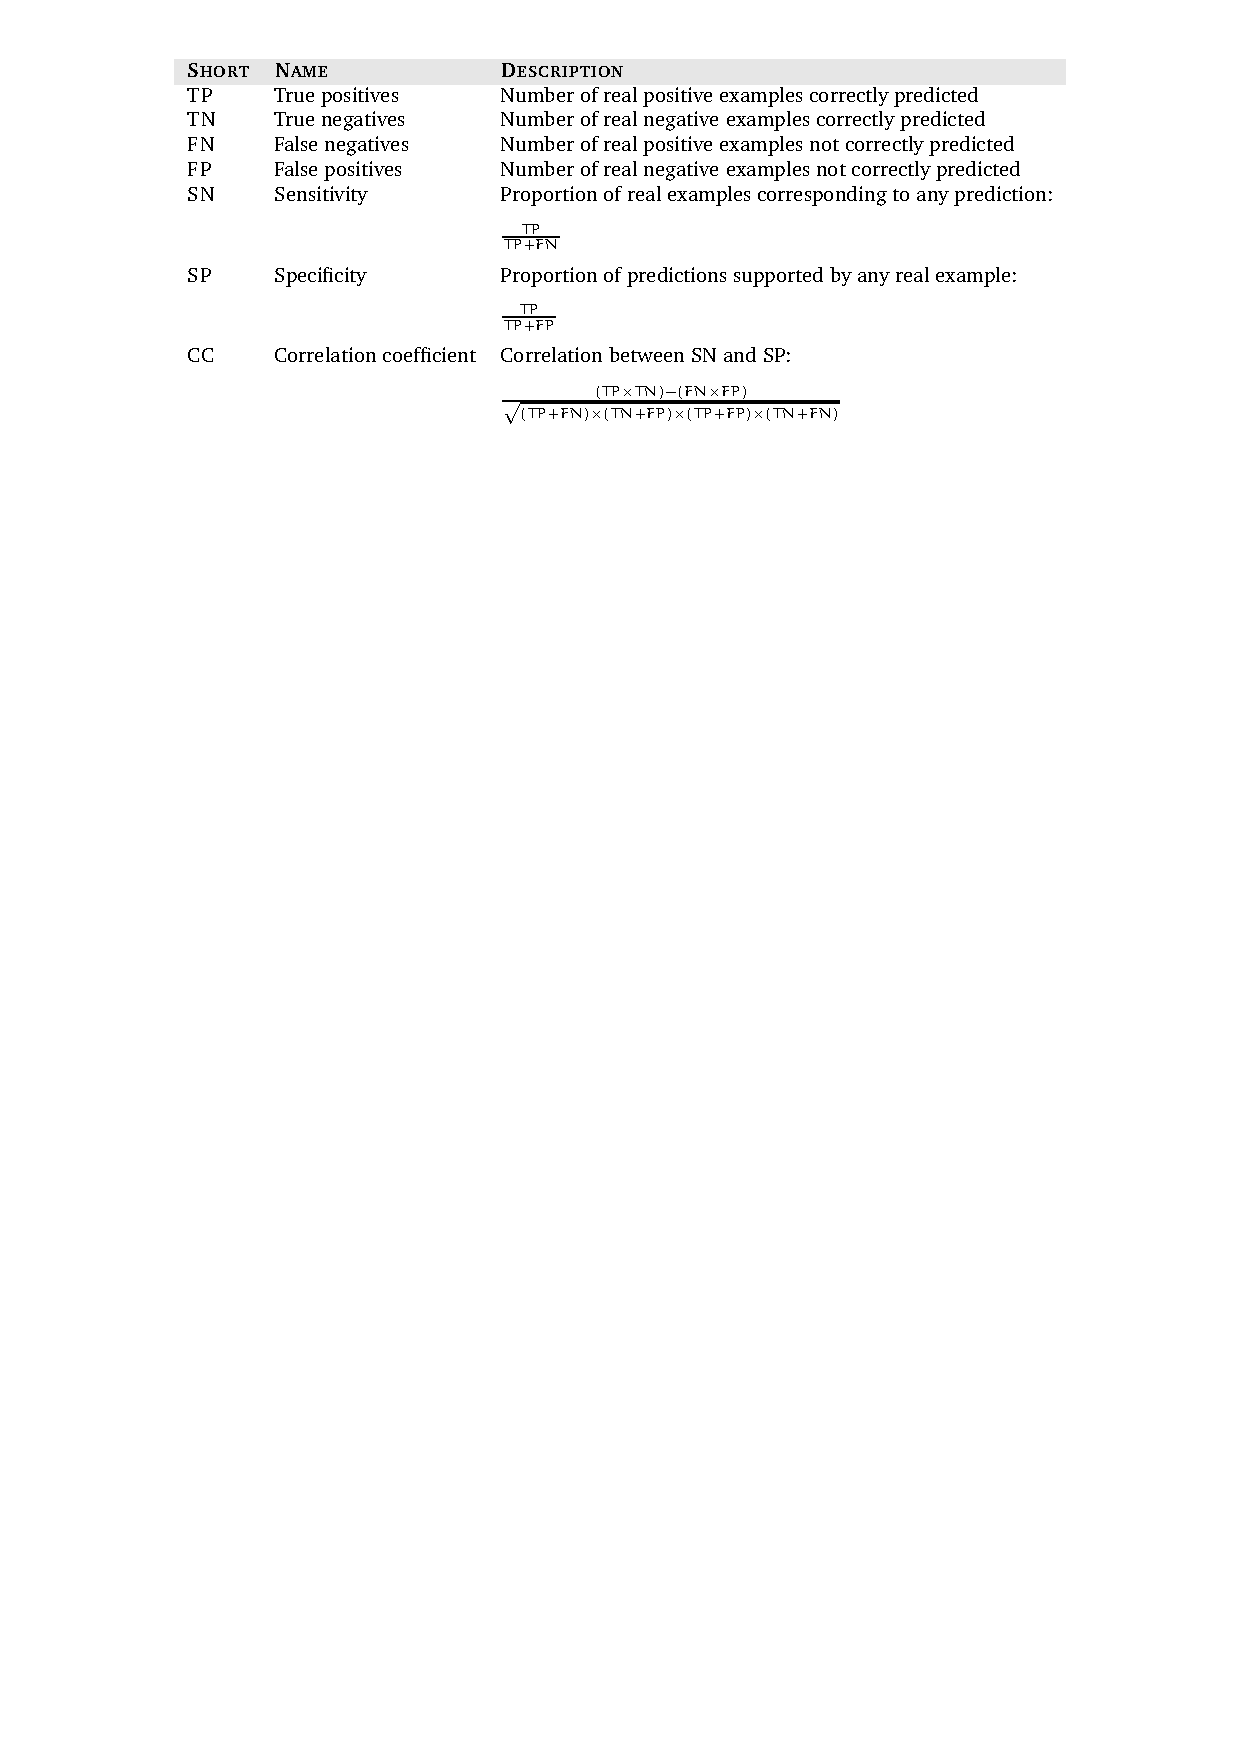
\includegraphics[bb=84 629 515 817,clip]{tables/accuracy}}
\end{center}
\end{minipage}
\mycaption{tab:accuracygenef}% label
          {The common accuracy measures in sequence analysis}% lof
          {The common accuracy measures in sequence analysis.}% caption header
          {}
\end{center}
\end{table}

Nowadays, after the completion of the first draft of the human genome 
we are completely immersed in a context of genomic research. The current generation 
of gene finders is devoted to the automatic reannotation of genomes by using the increasing 
amount of new information. Comparisons between genomes have proven to be very 
helpful in the discovery of novel genes \citep{guigo:2003a}. Some representatives
of the current generation of gene prediction programs are \prog{fgenesh+} 
\citep{salamov:2000a}, \prog{geneid} \citep{blanco:2003a} and \prog{genomescan} 
\citep{yeh:2001a}, or the comparative analysis systems \prog{doublescan} \citep{meyer:2002a}, 
\prog{rosetta} \citep{batzoglou:2000a}, \prog{slam} \citep{alexandersson:2003a}, 
\prog{sgp1} \citep{wiehe:2001a}, \prog{sgp-2} \citep{parra:2003a} 
and \prog{twinscan} \citep{korf:2001a}. 

The latest achievements in the sequencing of other higher eukaryotes have allowed the advent 
of comparative predictors that consider the alignment of multiple genomes in the prediction model, 
such as \prog{N-scan} that simultaneously combines the genomes of human, mouse, rat and 
chicken \citep{gross:2005a}. Moreover, new tools such as \prog{jigsaw} \citep{allen:2005a} and 
\prog{gaze} \citep{howe:2002a} for the assembly of data obtained from 
external sources of prediction and experimental evidence have been recently 
developed. 

\subsectionblue{\prog{geneid}}

\index{geneid}
The current version of \prog{geneid} \citep{blanco:2003a} is a program that predicts genes in anonymous 
genomic sequences designed following a simple hierarchical structure (see Figure \ref{fig:geneid} (A)). 
First, splice sites and start and stop codons are predicted and scored along the sequence. 
Next, potential exons are constructed from these sites and scored as the sum 
of the defining sites plus the score of a Markov model for coding DNA. Finally, 
from the set of predicted exons, the gene structure maximizing the sum of the 
score of its exons is assembled using a dynamic programming algorithm \citep{guigo:1998a}.

\prog{geneid} offers two features to integrate external information into the ab initio predictions: 
(1) sequence homology information can be used to reinforce the predictions that are supported by the 
alignment and (2) partial or complete genes obtained from other sources can be incorporated before 
the exon assembly.

As a consequence of its simple design, \prog{geneid} has been also parallelized.
Parallelism of data (distribution of data among processors with shared memory) was 
finally implemented because it was the best solution for distributing the
overload in the system. Following the divide and conquer strategy, the best gene 
structures computed in different processors are assembled introducing 
some overlap between sequence fragments (see Figure \ref{fig:geneid} (B)).

%%%%
% Figure 13: geneid + geneid parallel
%%%%
\begin{figure}[t!]
\begin{center}
\setlength{\fboxsep}{2pt}
\fbox{
\begin{tabular}{cc}
\incgraph{width=0.3\linewidth,height=6cm}{ps/geneid1} & 
\vspace{-1ex} \incgraph{width=0.55\linewidth,height=5cm}{ps/geneid2}\\
A & B \\
\end{tabular}}
\mycaption{fig:geneid}% label
          {\prog{geneid} dataflow}% lof
          {\prog{geneid} dataflow.}% caption header
          {(A) The serial dataflow. (B) The parallel dataflow.}
\end{center}
\end{figure}


The simplicity of the architecture of \prog{geneid} is appropriate to deal with
problems different from the canonical ones. Taking advantage of the implemented facilities to 
reannotate sequences, \prog{geneid} has been the main component of two recent genome annotation 
pipelines:

\begin{menumerate}
\item
Identification of novel selenoproteins in eukaryotes.\index{selenoproteins}
The presence of a secondary structure (SECIS element) in the 3' UTR of the mRNA induces the 
UGA codon, usually a termination signal, to be translated as Selenocysteine. \prog{geneid} was 
modified to permit the dual meaning of the UGA triplet, being succesfully applied to describe the 
\emph{Drosophila melanogaster}, human and \emph{Takifugu rubripes} selenoproteomes 
\citep{castellano:2001a, kryukov:2003a, castellano:2004a}. 
In addition, \prog{geneid} was used to reannotate selenoproteins in the \emph{Tetraodon nigroviridis} 
genome \citep{jaillon:2004a}, being the first eukaryotic genome project to integrate the 
identification of this particular family into the gene annotation pipeline.
\item
Comparative gene prediction.
\prog{sgp2} is a method to predict genes in a target genome sequence using the sequence of a
second informant or reference genome \citep{parra:2003a}. Essentially, \prog{sgp2} 
is a framework to integrate the search program \prog{tblastx} results with
\prog{geneid} predictions. The result of the \prog{tblastx} alignment of two sequences
is used by \prog{geneid} to rescore the exons supported by the alignment, 
penalizing the score of the others. \prog{sgp2} was successfully used in cooperation 
with another similar program called \ver{twinscan} \citep{korf:2001a} to discover 
a set of novel human and mouse genes. A subset of them was then experimentally 
validated in a subsequent stage of the genome comparison protocol \citep{guigo:2003a}.
The same protocol was used to annotate the genomes of human and chicken \citep{hillier:2004a}.
\end{menumerate}

\sectionorange{The state of the art in promoter characterization}

\index{promoter characterization!sta@state of the art}
The first algorithms of sequence alignment were enterely written to analyze proteins \citep{needleman:1970a}.
However, it was soon noticed that the same procedures could be applied over any type of biological
sequence, including transcription regulatory regions. For instance, \citet{sadler:1983a} used consensus 
and similarity searches to locate some general promoter elements in a set of vertebrate sequences. In 
\citep{waterman:1984d}, two algorithms to detect a common motif that can be known or unknown a priori 
in a set of sequences were presented. Later, these algorithms were used to characterize the 
core promoter of several \emph{Escherichia coli} genes \citep{galas:1985a}.

Consensus are a rudimentary form for representing regulatory sites so that new proposals to overcome their
limitations were published. \citet{staden:1984a} suggested the use of weight matrices. These PWMs were 
constructed from previous alignments of different types of biological sites. \citet{bucher:1990a}
systematically refined and tested the PWMs for detecting different regulatory 
signals such as the TATA box, the CAAT-box or the GC-box. At the same time, theoretical studies
to relate the information content and the quality of anchored alignments were already 
published \citep{schneider:1990a}. Posterior studies have shown the low specificity of the PWMs
when the set of initial examples is small \citep{schones:2005a}.

Soon, several databases to store the experimental examples and the constructed matrices were published, 
such as \db{Transfac} \citep{wingender:1988a}. At the same time, efficient programs to scan promoter 
sequences based on the pattern matching technique (pattern-driven approaches) were designed to use these 
matrices, being \prog{MatInspector} the most popular one \citep{frech:1993a,quandt:1995a}. However, methods 
to identify TFBSs in a single sequence demonstrated a very poor performance with an excess of false positives.
Certain improvements were observed when using additional information. New heuristic methods to discover 
unkown patterns in a set of regulatory sequences appeared (sequence-driven approaches): the application 
of the Gibbs sampling \citep{lawrence:1993a} and the expectation-maximization method \citep{bailey:1994a} 
are good examples. 

In general, however, the experimental investigation of a single promoter in all cell types where it can 
be active, under all conceivable conditions, at all possible developmental and cell-cyle stages, is 
in practice impossible. With this limitation in mind, the predictions obtained by any method must
be always very carefully evaluated to avoid the rejection of predicted functional sites that have not been 
experimentally annotated yet.

The identification of the core promoter regions and the annotation of the TSSs have also been two problems
associated to the problem of the TFBSs prediction. The presence of significantly over-expressed words or 
an unusual high percentage of CpG dinucleotides have traditionally been two measures of promoterness. 
For instance, \citet{davuluri:2001a} combined these two sensors with splicing detection to locate the first 
exon of a gene, predicting therefore the TSS position. Neural networks and genetic algorithms were used
in \citep{knudsen:1999a} to discriminate between promoter and non-promoter sequences. \citet{fickett:1997a}
reviewed the topic, showing the poor accuracy of most methods in the detection of the TSS. Word 
over-representations have been also used to study the 
association of adjacent TFBSs to form regulational modules or clusters with interesting results although 
the deciphering of a regulatory code seems still too complex \citep{beer:2004a,sharan:2003a,terai:2004a,thompson:2004a}. An example of such architectures is shown in Figure \ref{fig:modules}.

%%%%
% Figure 14: regulatory modules
%%%%
\begin{figure}[t!]
\begin{center}
\setlength{\fboxsep}{2pt}
\fbox{\incgraph{width=0.8\linewidth,height=6cm}{ps/modules}}
\mycaption{fig:modules}% label
          {Transcriptional regulatory module architectures}% lof
          {Transcriptional regulatory module architectures.}% caption header
          {Regulatory proteins and their gene targets are represented as blue circles and red boxes, respectively. Solid arrows indicate protein-DNA interactions, and genes encoding regulators are linked to their protein products by dashed lines. Adapted from \citep{harbison:2004a}.}
\end{center}
\end{figure}

A new revolution in the study of gene regulation began with the availability of genomic information and 
the possibility to work with abundant expression data. Phylogenetic footprinting, for instance, is a
new form of leaving a great fraction of false positives out \citep{duret:1997a,fickett:2000a}. 
Promising results have been obtained in several investigations \citep{blanchette:2002a,krivan:2001a,lenhard:2003a}. A review on phylogenetic footprinting can be found in \citep{wasserman:2004a}. 
Gene expression data from microarrays is the other great hope in the field to elaborate a regulatory map of 
human. Despite at the beginning, there was a boom of analysis of such data in different biological 
problems \citep{beltran:2003a,golub:1999a,shoemaker:2001a}, the difficulty to analyze and understand such 
an amount of data has been underscored in many occasions, though. The new generation of arrays based on 
chromatin immunoprecipitation promise to be an interesting method of prediction validation 
\citep{odom:2004a}. The combination of comparative genomics and expression data will become in a few years
the standard way to study a group of genes as in \citep{xie:2005a}.

Due to the poor results obtained when analyzing sequences to find pure binding motifs, intensive research 
has been performed in other areas to understand better the gene regulation problem. For instance, the 
association between CpG islands and promoters \citep{cuadrado:2001a}, DNA structure \citep{pedersen:1998a}, 
nucleosome positioning \citep{ioshikhes:1999a} or protein-DNA physical interactions \citep{halford:2004a}.

Similarly to the gene-finding accuracy tests, several assessments have been performed about the
quality of promoter characterization tools, always with discouraging results. The lack of stable
data sets of regulation sites, and the surprising difficulty to deal sometimes with orthologous sequences
are two causes that suggests the need for further improvement \citep{prakash:2005a,tompa:2005a}.

\sectionorange{Looking forward}

Despite the numerous advances in the basic algorithms of gene and promoter 
prediction and the unceasing flow of new data, the way to determine the exact number of 
genes in the human genome remains unclear \citep{pennisi:2003a} and the elaboration of a 
regulatory map of the human genome seems today an objective too ambitious \citep{wasserman:2004a}.

In the discipline of gene prediction, the same concepts have been applied since more than 20 years
ago. While the basic gene models have been improved to support comparative research, the definition
of a gene predicted by a gene-finder is still the same. It is true that some non-canonical gene 
structures are being slowly incorporated into the programs such as prediction of UTRs, alternative
splicing forms or selenoproteins \citep{brent:2004a}. Right now, the gene identification problem is 
still open and many efforts are engaged in the creation of a solid catalogue of human genes 
\citep{encode:2004a}, in which large-scale experimental methods of validation will be crucial \citep{brent:2005a}. 

Moreover, gene prediction and promoter recognition should be performed simultaneously. Unfortunately, 
we are far from reaching such an achievement due to the poor performance in the detection of regulatory elements 
despite the new and promising research that is currently being done in that direction \citep{pennacchio:2001a}.
The enormous volume of high-throughput expression data has provided new opportunities in the investigation of
the biology of the systems \citep{davidson:2002a}. Phylogenetic footprinting is also demonstrating their
capability to unveil regulatory blocks conserved in several species \citep{wasserman:2000a}. In addition, more accurate
catalogues of annotated regulatory elements are appearing, making the training of new pattern discovery methods
easier. All together will be part of a future pipeline to automatically identify and annotate the eukaryotic promoter 
regions. However, much effort must be still invested in understanding better other aspects of the same biological problem 
such as chromatin effect, methylation, or nucleosome movement \citep{pedersen:1999a}.

Perhaps a new line of thought should be established in both fields \citep{claverie:2000a}. So far, we have been only 
focusing on the sequence and many successful advances have been possible following such an approach. However, it is assumed that 
the cell machinery works in many levels with uncountable number of interactions that we have not incorporated 
in our systems yet. Once we have reached the limit with the current methods, and that moment is not too far, it will be 
essential to move from the current analytical systems to more constructive and dynamic applications, emulating
the mechanisms of the cell.

%%%%%%%%%%%%%%%%%%
%%% References for this chapter
%%% ENCERRAR ENTRE LLAVES PARA EVITAR PROBLEMAS
\bibliographystyle{plainnat}
{\bibliography{sections/bibliography}}
